\documentclass[aspectratio=169]{beamer}

\usepackage[utf8]{inputenc}
\usetheme{Madrid}
\usecolortheme{beaver}
\usepackage{fontspec}
\usepackage{listings}
\usepackage{fancyvrb}

%Information to be included in the title page:
\title{RESTful API Development using Go}
%\subtitle{}
\author{Baiju Muthukadan}
%\institute{Red Hat}
\date{@nogenerics}

\logo{
\includegraphics[height=1.5cm]{images/gopher4.png}}

\begin{document}
\beamertemplatenavigationsymbolsempty

\setmainfont
[ Path = ../fonts/,
UprightFont = DejaVuSerif.ttf,
ItalicFont = DejaVuSerif-Italic.ttf,
BoldFont = DejaVuSerif-Bold.ttf,
BoldItalicFont = DejaVuSerif-BoldItalic.ttf,
Numbers={Lining, Monospaced},
] {DejaVu Serif}

\setsansfont
[ Path = ../fonts/,
UprightFont = DejaVuSans.ttf,
ItalicFont = DejaVuSans-Oblique.ttf,
BoldFont = DejaVuSans-Bold.ttf,
BoldItalicFont = DejaVuSans-BoldOblique.ttf,
Numbers={Lining, Monospaced},
] {DejaVu Sans}

\setmonofont
[ Path = ../fonts/,
UprightFont = DejaVuSansMono.ttf,
ItalicFont = DejaVuSansMono-Oblique.ttf,
BoldFont = DejaVuSansMono-Bold.ttf,
BoldItalicFont = DejaVuSansMono-BoldOblique.ttf,
Numbers={Lining, Monospaced},
] {DejaVu Sans Mono}


\newfontfamily{\vollkorn}
[ Path = ../fonts/,
UprightFont = Vollkorn-Regular.otf,
ItalicFont = Vollkorn-Italic.otf,
BoldFont = Vollkorn-Bold.otf,
BoldItalicFont = Vollkorn-BoldItalic.otf,
Numbers={Lining, Monospaced},
] {Vollkorn}

\newfontfamily{\dejavuserif}
[ Path = ../fonts/,
UprightFont = DejaVuSerif.ttf,
ItalicFont = DejaVuSerif-Italic.ttf,
BoldFont = DejaVuSerif-Bold.ttf,
BoldItalicFont = DejaVuSerif-BoldItalic.ttf,
Numbers={Lining, Monospaced},
] {DejaVu Serif}

\newfontfamily{\dejavusans}
[ Path = ../fonts/,
UprightFont = DejaVuSans.ttf,
ItalicFont = DejaVuSans-Oblique.ttf,
BoldFont = DejaVuSans-Bold.ttf,
BoldItalicFont = DejaVuSans-BoldOblique.ttf,
Numbers={Lining, Monospaced},
] {DejaVu Sans}

\newfontfamily{\dejavumono}
[ Path = ../fonts/,
UprightFont = DejaVuSansMono.ttf,
ItalicFont = DejaVuSansMono-Oblique.ttf,
BoldFont = DejaVuSansMono-Bold.ttf,
BoldItalicFont = DejaVuSansMono-BoldOblique.ttf,
Numbers={Lining, Monospaced},
] {DejaVu Sans Mono}

\frame{\titlepage}

\begin{frame}[fragile]
  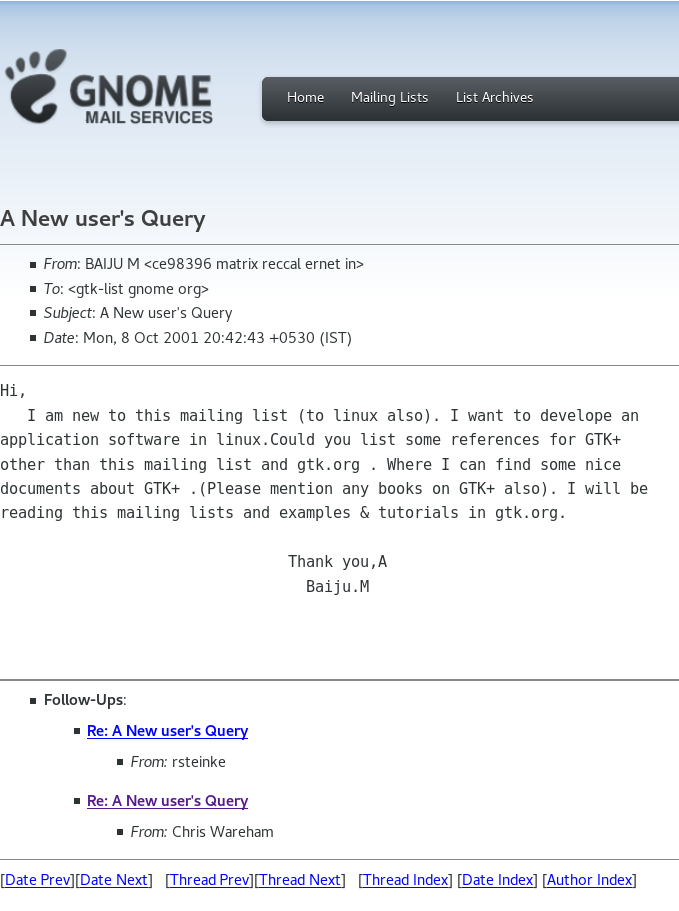
\includegraphics[scale=.25]{images/first-mail.png}
\end{frame}

\begin{frame}
  \frametitle{About Me}

  \begin{itemize}
  \item<1-> Senior Software Engineer, Red Hat
  \item<2-> FOSS Contributor (SMC, Koha, Zope, SaltStack, fabric8 etc.)
  \item<3-> Founded the Swathanthra Malayalam Computing (SMC) project in 2001 while studying at REC Calicut (NIT Kozhikode)
  \item<4-> Received the first Kenneth Gonsalves Award for contributions to the Python community in India
  \item<5-> Author of the book: A Comprehensive Guide to Go Programming \footnote{\url{https://golang.muthukadan.net}}
  \end{itemize}

\end{frame}

\begin{frame}
  \frametitle{Quick introduction to Go}

  \begin{itemize}
  \item<1-> General Purpose Programming Language
  \item<2-> Free/Open Source
  \item<3-> Created at Google by Robert Griesemer, Rob Pike and Ken Thompson
  \item<4-> Development started in 2007 and publicly released in November 2009
  \item<5-> C like syntax (no semicolons)
  \item<6-> Object Oriented (Composition over inheritance \- no classes!)
  \item<7-> Compiled (Statically linked)
  \item<8-> Garbage collected
  \item<9-> Statically typed
  \item<10-> Strongly typed

  \end{itemize}

\end{frame}
    
\begin{frame}
  \frametitle{Quick introduction to Go ...}
    
  \begin{itemize}
  \item<1-> built-in concurrency
  \item<2-> Two major compilers: gc \& gccgo
  \item<3-> 25 keywords (less than C,C++,Python etc.)
  \item<4-> Classification (Capitalized are exported \- public)
  \item<5-> Fast build (in seconds)
  \item<6-> Unused imports and variables raise compile error
  \item<7-> Operating Systems: Windows, GNU/Linux, Mac OS X, *BSD etc.
  \item<8-> CPU Architectures: amd64, 386, arm etc.
  \item<9-> Cross compilation
  \item<10-> Standard library
  \item<11-> No exceptions (Errors are values)
  \item<12-> Pointers (No pointer arithmetic!)

  \end{itemize}

\end{frame}

\begin{frame}[fragile]
  \frametitle{Basic example}

\begin{Verbatim}[fontsize=\small]
package main

import "net/http"

func main() {
        http.ListenAndServe(":8080", nil)
}
\end{Verbatim}

\end{frame}

\begin{frame}[fragile]
  \frametitle{Serve content example}

\begin{Verbatim}[fontsize=\small]
package main

import "net/http"

func homeHandler(w http.ResponseWriter, r *http.Request) {
        w.Write([]byte("Hello World!"))
}

func main() {
        http.HandleFunc("/", homeHandler)
        http.ListenAndServe(":8080", nil)
}
\end{Verbatim}

\end{frame}


\begin{frame}[fragile]
  \frametitle{Gorilla Mux}

  \begin{itemize}
  \item URL router and dispatcher
  \item \url{http://www.gorillatoolkit.org/pkg/mux}
  \item \url{https://github.com/gorilla/mux}
  \end{itemize}

\begin{Verbatim}[fontsize=\small]
go get -u github.com/gorilla/mux
\end{Verbatim}
  
\end{frame}


\begin{frame}[fragile]
  \frametitle{Gorilla Mux Example}

\begin{Verbatim}[fontsize=\small]
package main

import (
        "net/http"
        "github.com/gorilla/mux"
)

func homeHandler(w http.ResponseWriter, r *http.Request) {
        w.Write([]byte("Hello World!\n"))
}

func main() {
        r := mux.NewRouter()
        r.HandleFunc("/", homeHandler).Methods("GET")
        http.Handle("/", r)
        http.ListenAndServe(":8080", nil)
}
\end{Verbatim}
  
\end{frame}

\begin{frame}[fragile]
  \frametitle{Negroni Example}

\begin{Verbatim}[fontsize=\small]
func main() {
        r := mux.NewRouter()
        r.HandleFunc("/", homeHandler)
        n := negroni.New()
        n.UseHandler(r)
        http.ListenAndServe(":8080", n)
}
\end{Verbatim}
\end{frame}

\begin{frame}[fragile]
  \frametitle{Negroni Middleware}

  An exaple from \small{\url{https://github.com/kaaryasthan/kaaryasthan/blob/master/route/route.go}}
  
\begin{Verbatim}[fontsize=\small]
n = negroni.New(negroni.NewRecovery(),
                negroni.NewLogger(),
                negroni.NewStatic(web.AssetFS()))
n.Use(middleware)
\end{Verbatim}
Middlewares: gzip, jwt, cors, csp
\end{frame}


\begin{frame}[fragile]
  \frametitle{Paths with variable}

  \begin{Verbatim}[fontsize=\small]
    r := mux.NewRouter()
    r.HandleFunc("/products/{key}", ProductHandler)
    r.HandleFunc("/articles/{category}/", ArticlesCategoryHandler)
    r.HandleFunc("/articles/{category}/{id:[0-9]+}", ArticleHandler)
\end{Verbatim}

  Format:
  \texttt{ \{name\} or \{name:pattern\}}

\end{frame}

\begin{frame}[fragile]
  \frametitle{Frameworks}

  \begin{itemize}
  \item \url{https://gobuffalo.io}
  \item \url{https://goa.design}
  \item \url{https://gin-gonic.github.io/gin}
  \item \url{https://beego.me}
  \item \url{https://awesome-go.com/#web-frameworks}
  \end{itemize}

\end{frame}

\begin{frame}[fragile]
  \frametitle{RESTful}

  \begin{itemize}
  \item stateless
  \item unique identification of resources through URIs
  \item standard HTTP methods (POST, GET, PATCH, DELETE)
  \item HTTP status codes
  \end{itemize}
  
\end{frame}

\begin{frame}[fragile]
  \frametitle{Why RESTful?}

  \begin{itemize}
  \item easy to understand \& document
  \item works on limited bandwidth
  \item READs can be cached and hence reduces the bandwidth
  \end{itemize}
  
\end{frame}

\begin{frame}[fragile]
  \frametitle{Architecture constraints}

  \begin{itemize}
  \item uniform interface
  \item client-server
  \item stateless
  \item Cache-able
  \item Layered system
  \end{itemize}
  
\end{frame}

\begin{frame}[fragile]
  \frametitle{REST Style consists of ...}

  \begin{itemize}
  \item Resources
  \item Verbs
  \item Media types
  \item Status codes
  \end{itemize}
  
\end{frame}

\begin{frame}[fragile]
  \frametitle{Media types}

  Use JSON ( \url{http://json.org} )

  or better JSON API SPEC ( \url{http://jsonapi.org} )

  \texttt{application/vnd.api+json}
  
\end{frame}

\begin{frame}[fragile]
  \frametitle{Authentication}

  Use JWT: https://jwt.io
  
\end{frame}

\begin{frame}[fragile]
  \frametitle{Security}

  All attacks possible with web are applicable to REST API.
  
  https://www.owasp.org

  - Use TLS always
  
\end{frame}

\begin{frame}[fragile]
  \frametitle{Tooling}

  cURL is your friend!
  
\end{frame}


\begin{frame}[fragile]
  \frametitle{HTTP Methods}

  \begin{itemize}
  \item POST - Create
  \item GET - Read
  \item PATCH - Update
  \item DELETE - Delete
  \end{itemize}
  
\end{frame}

\begin{frame}[fragile]
  \frametitle{An example API end points}

  \begin{itemize}
  \item Create item - POST /items
  \item Read a single item - GET /items/1
  \item Read all items - GET /items
  \item Update item - PATCH /items/1
  \item Delete item - DELETE /items/1
  \end{itemize}

\end{frame}


\begin{frame}[fragile]
  \frametitle{API versioning}

  /api/v1/items

  /api/v2/items
  
\end{frame}

\begin{frame}[fragile]
  \frametitle{jsonapi.org}

  \begin{itemize}
  \item standard for representation of JSON responses
  \item shared convention increase productivity through generalized tooling
  \end{itemize}
  
\end{frame}

\begin{frame}[fragile]
  \frametitle{resource representation in JSON}

  \begin{Verbatim}[fontsize=\tiny]
  {
  "links": {
    "self": "http://example.com/articles",
    "next": "http://example.com/articles?page[offset]=2",
    "last": "http://example.com/articles?page[offset]=10"
  },
  "data": [{
    "type": "articles",
    "id": "1",
    "attributes": {
      "title": "JSON API paints my bikeshed!"
    },
    "relationships": {
      "author": {
        "links": {
          "self": "http://example.com/articles/1/relationships/author",
          "related": "http://example.com/articles/1/author"
        },
        "data": { "type": "people", "id": "9" }
      },
  ...
  \end{Verbatim}


\end{frame}

\begin{frame}[fragile]
  \frametitle{HTTP Status codes and Location header}

  \begin{itemize}
  \item If a POST request did not include a Client-Generated ID and
    the requested resource has been created successfully, the server
    MUST return a 201 Created status code.

  \item The response SHOULD include a Location header identifying the
    location of the newly created resource.
  \end{itemize}

\end{frame}

\begin{frame}[fragile]
  \frametitle{structure for errors}

  \begin{Verbatim}[fontsize=\tiny]
HTTP/1.1 422 Unprocessable Entity
Content-Type: application/vnd.api+json

{
  "errors": [
    {
      "status": "422",
      "source": { "pointer": "/data/attributes/first-name" },
      "title":  "Invalid Attribute",
      "detail": "First name must contain at least three characters."
    }
  ]
}
  \end{Verbatim}

\end{frame}

\begin{frame}
  \frametitle{Conclusion}

  Go is a great choice for RESTful API development\!

\end{frame}

\begin{frame}
  \begin{center}
    {\huge Thank You!}\\[1cm]
    {\large \href{https://twitter.com/nogenerics}{@nogenerics}}
  \end{center}
\end{frame}

\end{document}
